\externaldocument{chapter6}
\chapter{Analysis of Failure-Domain by ADFD+ and Daikon}
\label{chap:ADFD+}

\section{Introduction}\label{sec:intro6}
Testing is an essential and most widely used method for verification and validation process. Efforts have been continuously made by researchers to make it more and more effective and efficient. Testing is effective when it finds maximum number of faults in minimum number of test cases and efficient when it executes maximum number of test cases in minimum possible time. Upgrading existing techniques and developing new test strategies focus on increasing test effectiveness while automating one or more components or complete system aims at increasing efficiency.

Boundary Value Analysis (BVA) is one of the technique used of increasing test effectiveness. In BVA test cases with boundary values are added to the test suite with the assumption that errors reside along the boundaries~\cite{radatz1990ieee}. Daikon~\cite{ernst2007daikon} is an automatic tool used to improve the efficiency. It saves testers time by automatically generating likely program invariants.

However, the two approaches can adversely affect the testing process if wrong boundaries or invariants are taken into consideration. It is therefore motivating to accurately identify the boundaries of the input domain in BVA and measure the degree of correctness of auto-generated invariants by Daikon in the case of point, block and strip failure domain. To analyse the failure domains the ADFD+ technique was developed and experiments were conducted by testing several error-seeded one and two-dimensional numerical programs with ADFD+ and Daikon. The results obtained were analysed and reported.  

The main contributions of the study are:
\begin{itemize}
\item \textbf{ADFD+:} It is an extension of Automated Discovery of Failure Domain (ADFD) strategy developed by Ahmad and Oriol~\cite{ahmad2013adfd}. The new technique improves the search algorithm of ADFD and makes the report more intuitive (Section~\ref{sec:intro6_2}).
\item \textbf{Implementation of ADFD+:} It is implemented and integrated in the York Extensible Testing Infrastructure (Section~\ref{sec:intro6_4}).
\item \textbf{Evaluation:} The results generated by ADFD+ and Daikon about failure domains in the error-seeded programs are evaluated (Section~\ref{sec:intro6_7}). The results show that although Daikon generate invariant to identify the failure yet it is not able to identify the boundary of failure domain as accurately as ADFD+. 
\item \textbf{Future work:} ADFD+ can be extended to find and plot failure domains in multi-dimensional non-numerical programs (Section~\ref{sec:intro6_15}).
% A case study suggesting that boundaries are properly recognized by Daikon and ADFD+ or Daikon lake .... etc.
\end{itemize}
%The rest of this paper is organised as follows: \\ Section~\ref{sec:adfd} describes the ADFD+ strategy. Section~\ref{sec:imp} presents implementation of the ADFD+ strategy. Section~\ref{sec:eval} explains the experimental setup. Section~\ref{sec:res} shows results of the experiments. Section~\ref{sec:discussion} discusses the results. Section~\ref{sec:rw} presents related work and Section~\ref{sec:conc}, concludes the study.


%In the later part we plot the domain on the basis of invariants generated by Daikon and compare both the domains.

%%%%%%%%%%%%%%%%%    Background   %%%%%%%%%%%%%%%%%%%

\section{Preliminaries}\label{sec:intro6_1}
A number of empirical evidence confirms that failure revealing test cases tend to cluster in contiguous regions across the input domain~\cite{finelli1991nasa, schneckenburger2007towards, white1980domain}. According to Chan et al.~\cite{chan1996proportional} the clusters are arranged in the form of point, block and strip failure domain. In the point domain the failure revealing inputs are stand-alone, and spread through out the input domain. In block domain the failure revealing inputs are clustered in one or more contiguous areas. In strip domain the failure revealing inputs are clustered in one long elongated area. 

%\begin{figure}[ht]                                    
%\centering
%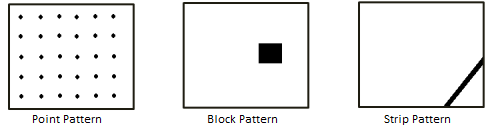
\includegraphics[width=12cm,height=4cm]{chapter6/ART_Patterns.png}
%\caption{Failure domains across input domain~\cite{chan1996proportional}}
%\label{fig:failurePatterns}
%\end{figure}

%In Section~\ref{sec:adfd+} we describe the ADFD+ framework that can find the failure, its domain and plot the domain up to the specified range in a graphical form. Experiments confirms the successful working of ADFD+.


 

%%%%%%%%%%%%%%%%%    ADFD+   %%%%%%%%%%%%%%%%%%%

\section{Automated Discovery of Failure Domain+}\label{sec:adfd+}\label{sec:intro6_2}
ADFD+ is an improved and extended form of ADFD strategy developed previously by Ahmad and Oriol~\cite{ahmad2013adfd}. It is an automated framework which finds the failures and their domains within a specified range and present them on a graphical chart. 

The main improvements of ADFD+ over ADFD strategy are stated as follows.

\begin{itemize}
\item ADFD+ generates a single Java file dynamically at run time to plot the failure domains as compared to one Java file per failure in ADFD. This saves sufficient time and makes the execution process quicker.

\item ADFD+ uses (x, y) vector series to represent failure domains as opposed to the (x, y) line series in ADFD. The vector series allows more flexibility and clarity to represent a failure and its domain.   

\item ADFD+ takes a single value as range with in which the strategy search for a failure domain whereas ADFD takes two values for lower and upper bound representing x and y-axis respectively.

\item In ADFD+, the algorithm of dynamically generating Java file, created at run-time after a failure is detected, is made more simplified and efficient.

\item In ADFD+, the failure domain is focused in the graph, which gives a clear view of, pass and fail points. The points are also labelled for clarification as shown in Figure~\ref{fig:Workflow}. 

%The difference in representation of fault by ADFD and ADFD+ can be seen in figure .... Figure x is generated by ADFD with lower bound as ... and upper bound as ... While Figure Y is generated by ADFD+ with range ... for the same program given in appendix a. 
\end{itemize}


%%%%%%%%%%%%%%%%%%%%

\subsection{Workflow of ADFD+}\label{sec:intro6_3}
ADFD+ is a completely automatic process and all the user has to do is to specify the program to test and click the $Draw Fault Domain$ button. The default value for range is set to 5, which means that ADFD+ will search 83 values around the failure. On clicking the button YETI is executed with ADFD+ strategy to search for a failure in two-dimension program. On finding a failure the ADFD+ strategy creates a Java file which contains calls to the program on the failing value and its surrounding values within the specified range. The Java file is compiled and executed and the result is analysed to check for pass and fail values. Pass and fail values are stored in pass and fail text files respectively. At the end of test, all the values are plotted on the graph with pass values in blue and fail values in red colour as shown in Figure~\ref{fig:Workflow}.
\\

%Instead of front end give workflow. It will make more sense. Change the code of the program

\begin{figure}[ht]
\centering
\includegraphics[width= 14cm,height=10cm]{chapter6/adfdPlusWorkflow.png}
\caption{Workflow of ADFD+}
\label{fig:Workflow}
\end{figure}


%%%%%%%%%%%%%%%%%%%%
%ADFD+ is an extension of ADFD's algorithm with more accuracy to find and clarity to plot the failure domain on a graphical chart. Deriving failure domains using ADFD+ is a one click process and all the tester needs to input is the class to test and the range-value for which to search around the found failure. 
%%%%%%%%%%%%%%%%%%%%

\subsection{Implementation of ADFD+}\label{sec:intro6_4}
The ADFD+ technique is implemented in YETI. The tool YETI is available in open-source at \url{http://code.google.com/p/yeti-test/}. A brief overview of YETI is given with the focus on parts relevant to implementation of ADFD+ strategy.

YETI is a testing tool developed in Java that tests programs using random strategies in an automated fashion. YETI meta-model is language-agnostic which enables it to test 
programs written in functional, procedural and object-oriented languages. 

YETI consists of three main parts including core infrastructure for extendibility, strategies section for adjustment of multiple strategies and 
languages section for supporting multiple languages. Both strategies and languages sections have pluggable architecture to easily incorporate new strategies and 
languages making YETI a favourable choice to implement ADFD+ strategy. YETI is also capable of generating test cases to reproduce the failures found during the test session. 
The strategies section in YETI contains all the strategies including random, random+ and DSSR to be selected for testing according to the specific needs. The default test 
strategy for testing is random. In strategies package, on top of the hierarchy, is an abstract class $YetiStrategy$, which is extended by $YetiRandomPlusStrategy$ and is further extended to get ADFD+ strategy.

\begin{figure*}[ht]
\centering
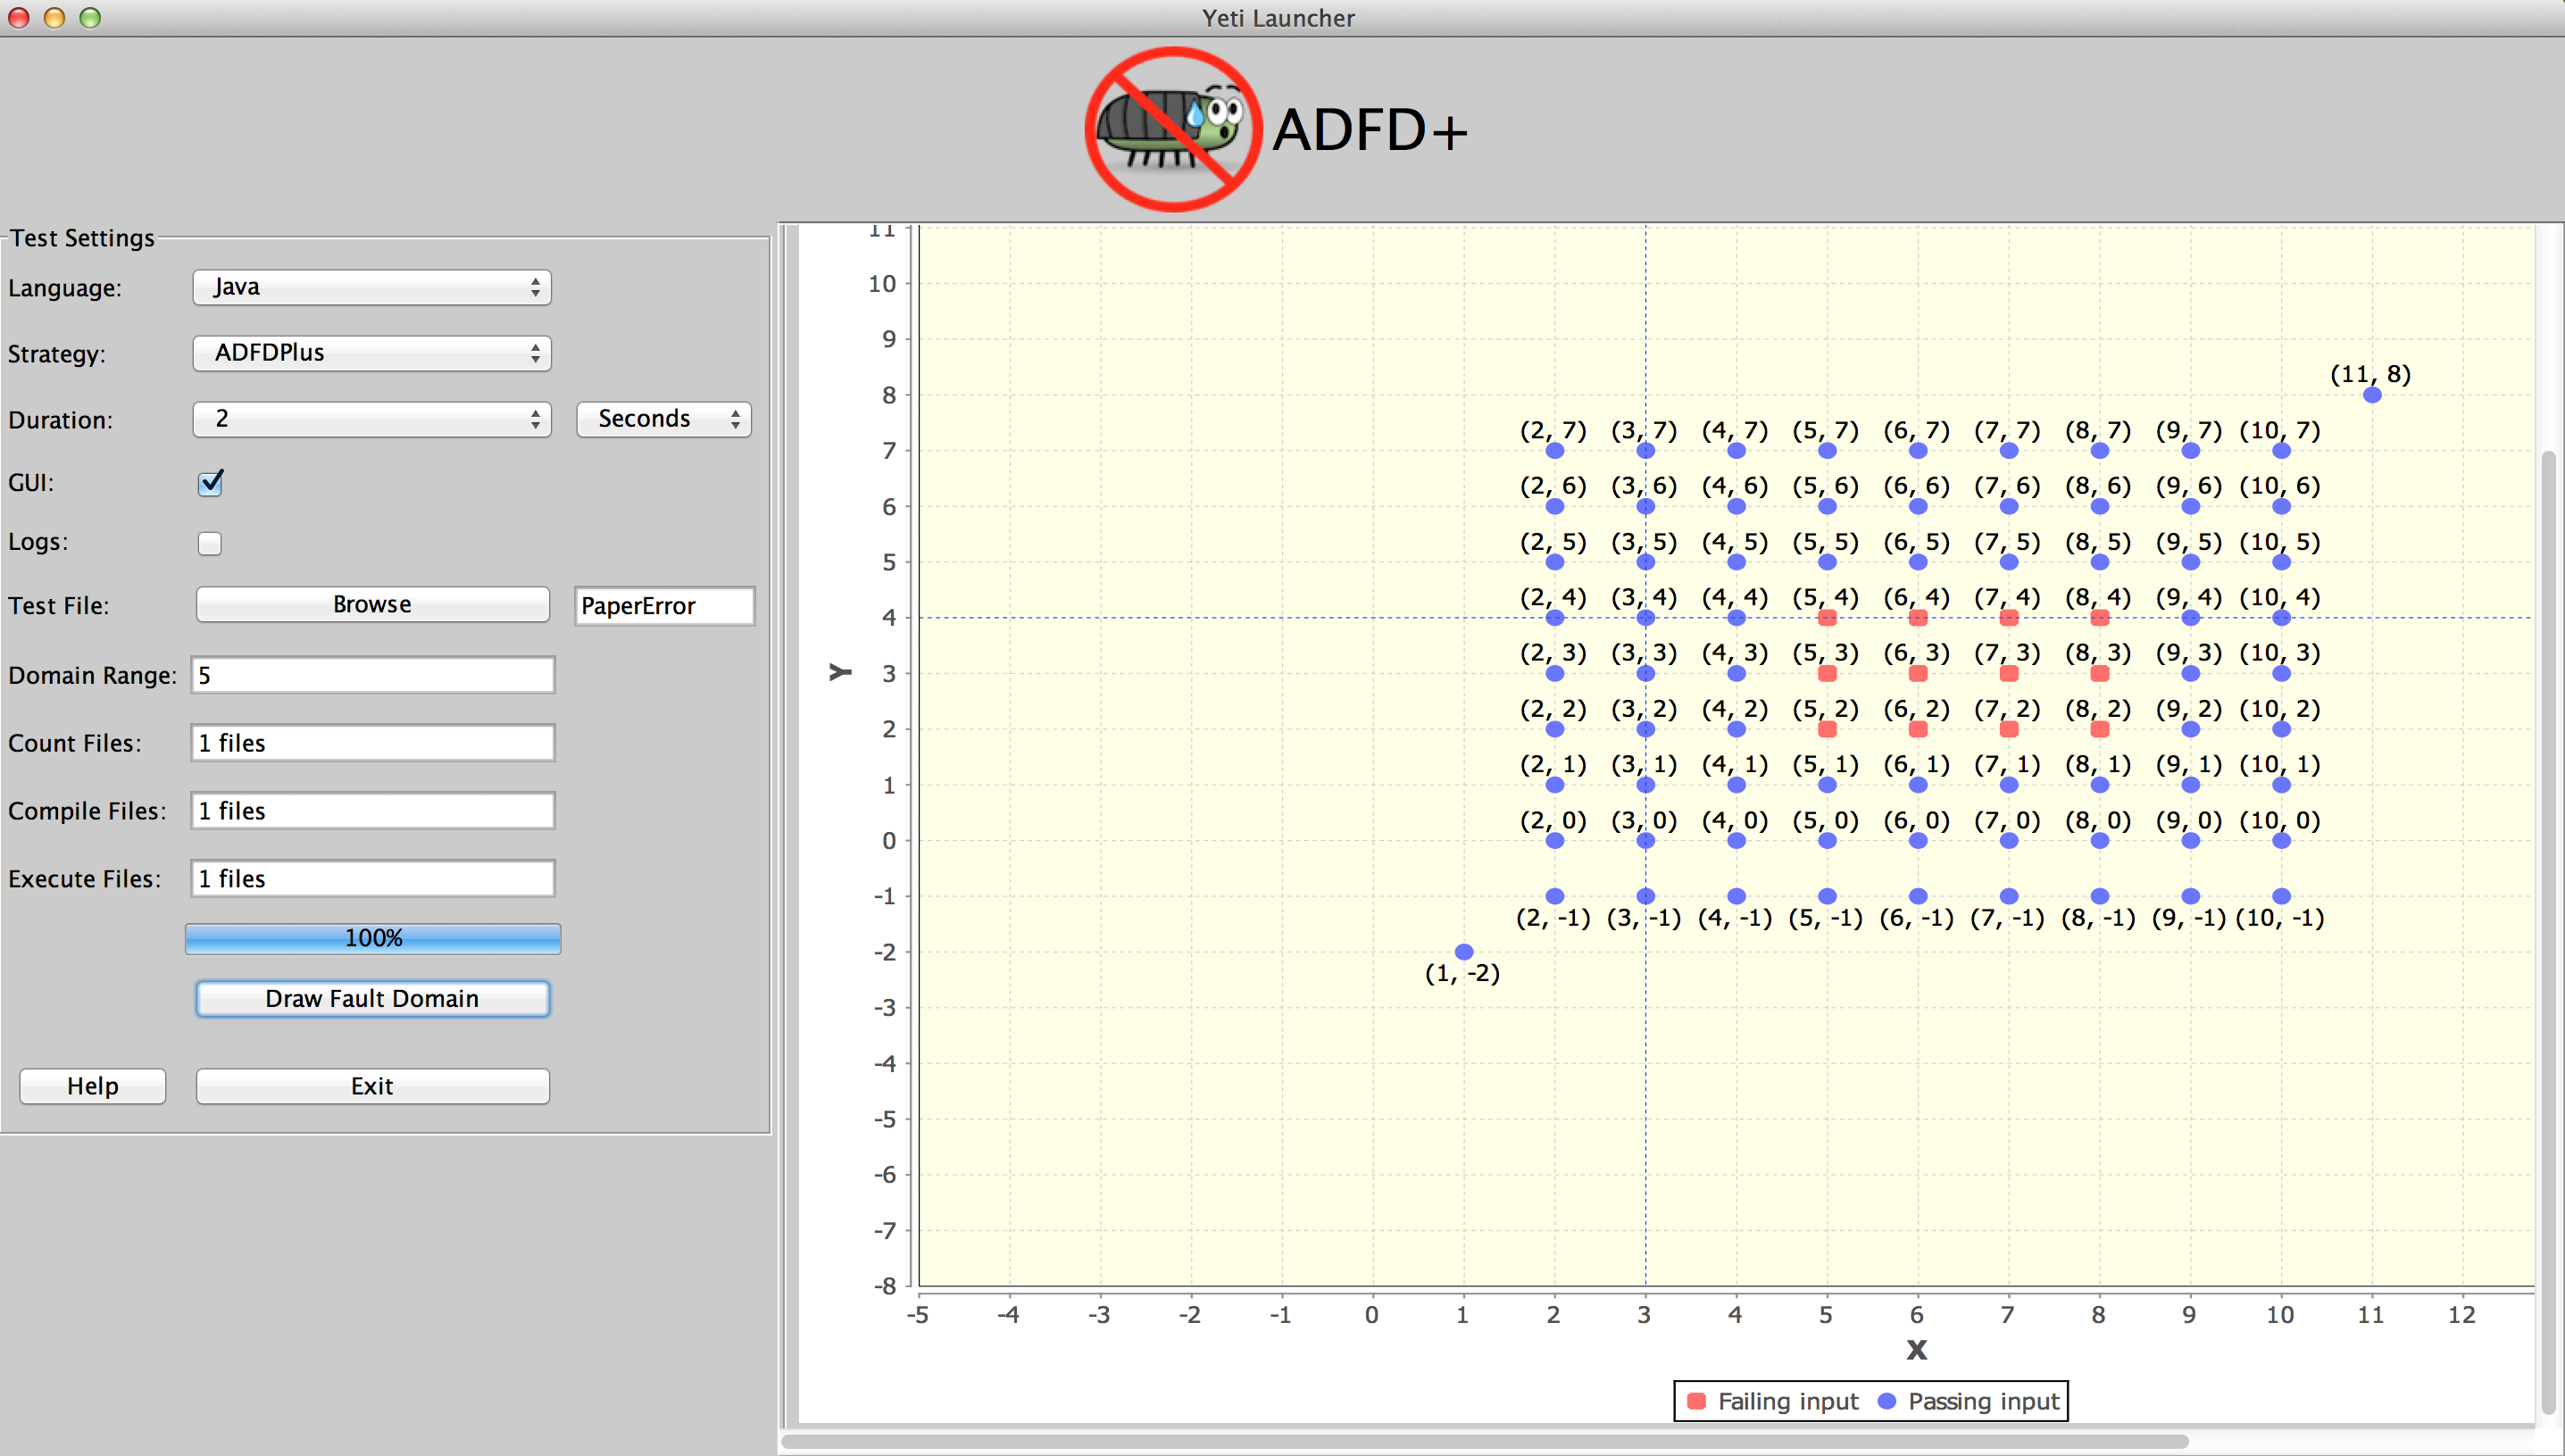
\includegraphics[width=15.5cm,height=11cm]{chapter6/exampleError.png}
\caption{The output of ADFD+ for the above code.}
\label{fig:adfdPlusExample}
\end{figure*}

\subsection{Example to Illustrate Working of ADFD+}\label{sec:intro6_5}
Suppose we have the following error-seeded class under test. From the program code, it can be easily noticed that an $ArithmeticException$ (DivisonByZero) failure is generated when the value of variable $x$ ranges between 5 to 8 and the value of variable $y$ between 2 to 4.

\begin{lstlisting}

public class Error {

  public static void Error (int x, int y){

    int z;

    if (((x>=5)&&(x<=8))&&((y>=2)&&(y<=4)))
		 {
			 z = 50/0;
		 }
   } 
}
\end{lstlisting}

On test execution, the ADFD+ strategy evaluates the class with the help of YETI and finds the first failure at x = 6 and y = 3. Once a failure is identified ADFD+ uses the surrounding values around it to find a failure domain. The range of surrounding values is limited to the value set by the user in the $Domain Range$ variable. When the value of $Domain Range$ is 5, ADFD+ evaluates total of 83 values of $x$ and $y$ around the found failure. All evaluated (x, y) values are plotted on a two-dimensional graph with red filled circles indicating fail values and blue filled circles indicating pass values. Figure~\ref{fig:adfdPlusExample} shows that the failure domain forms a block pattern and the boundaries of the failure are $(5, 2), (5, 3),(5, 4), (6, 2), (6, 4), (7, 2), (7, 4), (8, 2), (8, 3), (8, 4)$. 





%%%%%%%%%%%%%%%%%%%%%%%%%%%%%%%%%%%%%%%%%%%%%%%%%

\section{Daikon}\label{sec:intro6_6}
Daikon is a tool~\cite{ernst2007daikon}, which uses machine-learning technique to automatically generate likely invariants of the program written in C, C++, Java and Pearl. Daikon takes the program and a few test cases as input. The test cases may be either generated manually or by an automated tool. Daikon executes the test cases on the program under test and observes the values that the program computes. At the end of the test session it reports the properties that were true for the observed executions. A feature of Daikon facilitate to process the generated invariants to mitigate non-interesting and redundant invariants. Another feature allows to inserts the generated invariants in to the source code as assertions. The report generated by Daikon is useful in understanding program logic, generating invariants, predicting incompatibilities in component integration, automating theorem proving, repairing inconsistencies in data structures and checking the validity of data streams.




%%%%%%%%%%%%%%%%%    EVALUATION   %%%%%%%%%%%%%%%%%%%%


\section{Evaluation of Daikon by ADFD+}\label{sec:intro6_7}
Because of using error-seeded one and two dimensional numerical programs, we were aware of the failure domain present in each program. The correct identification and presentation of the failure domain by ADFD+ prove the correct working of ADFD+. We then evaluated the same program by Daikon and plot its results. The unit test cases required by Daikon for generating invariants were generated using Randoop~\cite{pacheco2007randoop}. YETI being capable of generating the test cases is not used for this step to keep the second completely independent from first. 

\subsection{Research Questions}\label{sec:intro6_8}
The following research questions have been addressed in this study:
\begin{enumerate}
\item Is Daikon capable of generating invariants to identify the failure?
\item Is Daikon capable of generating invariants to identify the failure domain?
\item Is Daikon capable of generating invariants to identify the boundaries of the failure domain?
\end{enumerate}

\subsection{Experimental Setup}\label{sec:intro6_9}
To evaluate the performance of Daikon, we carried out testing of several error-seeded one and two-dimensional numerical programs written in Java. The programs were divided in to two sets. Set A and B contains one and two-dimensional programs respectively. Each program was injected with at least one failure domain of point, block or strip nature. Every program was tested independently for 30 times by both ADFD+ and Daikon. The external parameters were kept constant in each test run and the initial test cases required by Daikon were generated by using an automated testing tool Randoop. The code for the programs under test is given in Appendix~\ref{sec:appendix1} while the test details are presented in Table~\ref{table:ADFD+Results_6}. 

Every class was evaluated through $10^5$ calls in each test session of ADFD+.
%\footnote{The total number of tests is equal to $60\times 30\times 3 \times 10^5 = 540\times10^6~tests$.} 
Due to the absence of contracts and assertions in the code under test, undeclared exceptions were taken as failures in accordance with the previous studies~\cite{ahmad2013adfd, Oriol2011yeti}. All tests were performed with a 64-bit Mac OS X Lion Version 10.7.4 running on 2 x 2.66 GHz 6-Core Intel Xeon processor with 6 GB (1333 MHz DDR3) of RAM. YETI runs on top of the Java\texttrademark  SE Runtime Environment [version 1.6.0\_35]. The machine took approximately 100 hours to process the experiments.

\section{Results}

The results are split in to four sub-sections for convenience. 


\subsection{Test of One-dimension Programs by ADFD+}\label{sec:intro6_10}
In each of the 30 experiments, The ADFD+ successfully discovered and plotted the failure domains for point, block and strip pattern as shown in the Figure~\ref{fig:failureDomainsOneDimension_6}. The range value for each experiment was set to 100.

\begin{figure} [H]
\centering
\subfigure[Point failure domain in one-dimension]{
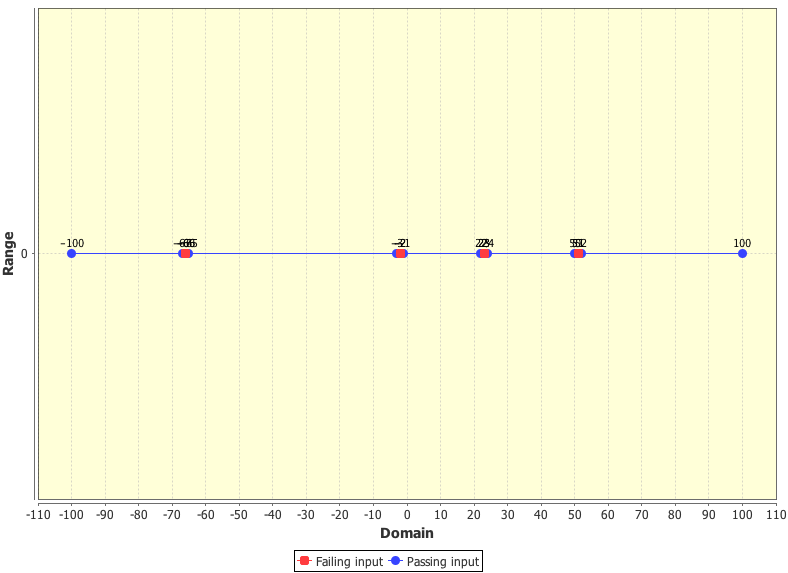
\includegraphics[width=14cm,height=6.2cm]{chapter6/PFDOne.png}
\label{fig:PFDOne_6}
}
\subfigure[Block failure domain in one-dimension]{
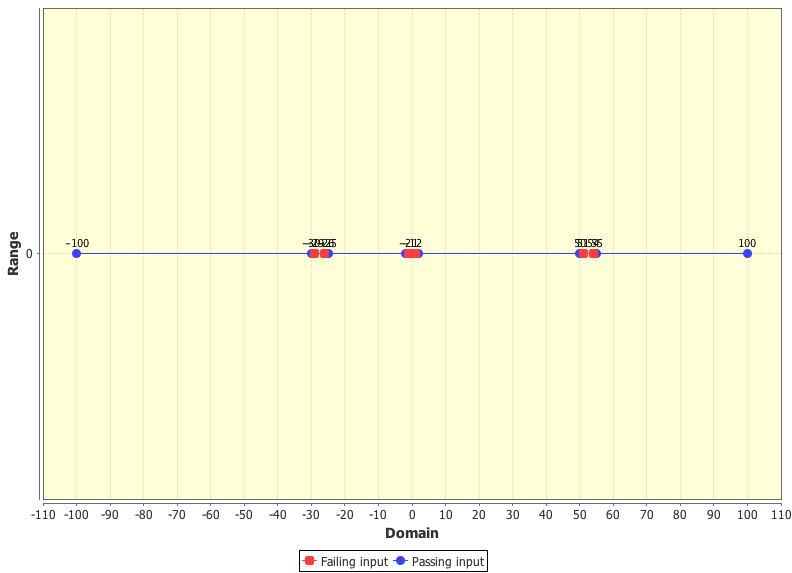
\includegraphics[width=14cm,height=6.2cm]{chapter6/BFDOne.png}
\label{fig:BFDOne_6}
}
\subfigure[Strip failure domain in one dimension]{
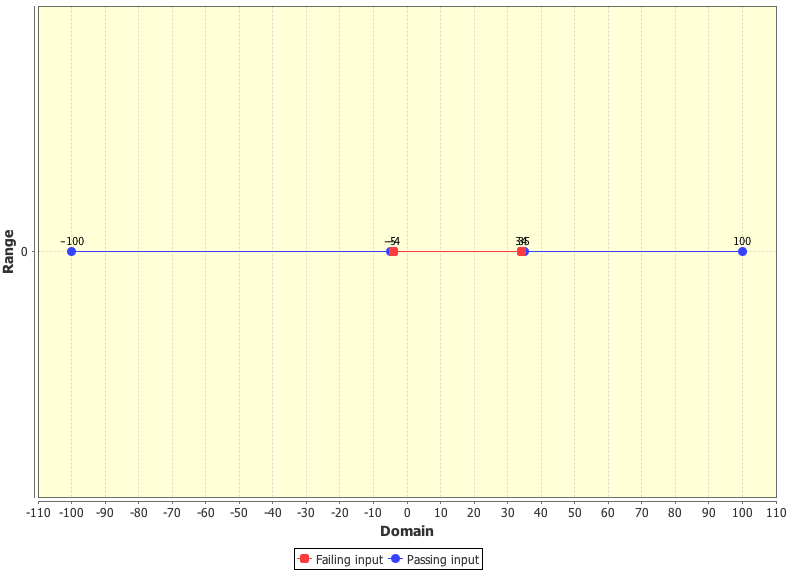
\includegraphics[width=14cm,height=6.2cm]{chapter6/SFDOne.png}
\label{fig:SFDOne_6}
}
\caption{Pass and fail values plotted by ADFD+ for one-dimension programs}

\label{fig:failureDomainsOneDimension_6}
\end{figure}
\begin{table}[h]
\caption{Table depicting values of x and y arguments responsible for forming point, block and strip failure domain in Figure \ref{fig:failureDomainsOneDimension_6}}
\bigskip
\centering
{\renewcommand{\arraystretch}{1.3}
\begin{tabular}{|l|l|l|}
\hline
Point failure		& 	Block failure		& 	Strip failure		\\
\hline
x =~-66			&	x =~-1			&	x = -4 --- 34 	\\	
x =~~-2		 	&	x =~~0			&					\\	
x =~~51 		&	x =~~1			&					\\
x =~~23 		& 	 				& 					\\
\hline
\end{tabular}
}
\bigskip
\label{table:failureDomains_6}
\end{table}



\subsection{Test of One-dimension Programs by Daikon}










\subsection{Test of Two-dimension Programs by ADFD+}\label{sec:intro6_11}
In each of the 30 experiments, The ADFD+ once again successfully discovered and plotted the failure domain for point, block and strip failure domain as shown in the Figure~\ref{fig:failureDomainsTwoDimension_6}. The range value for each experiment is set to 10. Labels are disabled in the charts given in Figure~\ref{fig:failureDomainsTwoDimension_6} for clarity purpose. The failure values in each of the point, block and strip failure domain is given in Table~\ref{table:failureDomains_6}. 

\begin{figure} [H]

\subfigure[Point failure domain in two-dimension]{
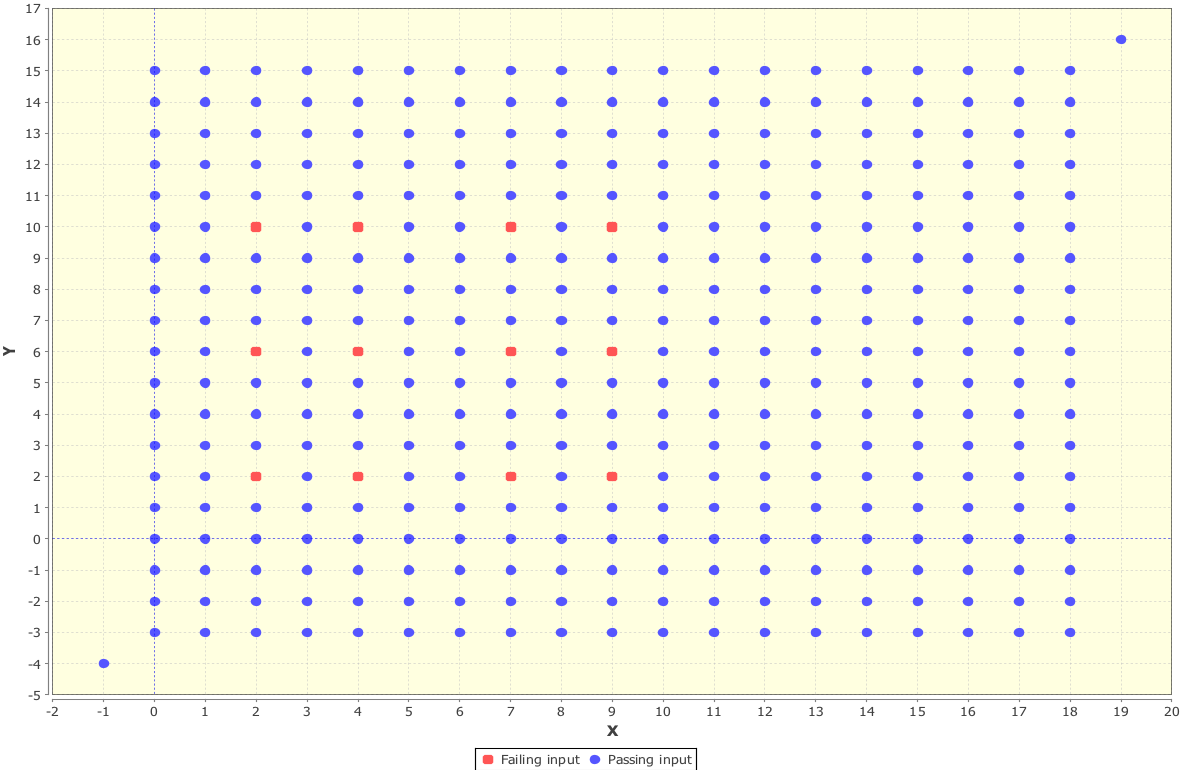
\includegraphics[width=14cm,height=6.2cm]{chapter6/PFDTwo.png}
\label{fig:PFDOne}
}
\subfigure[Block failure domain in two-dimension]{
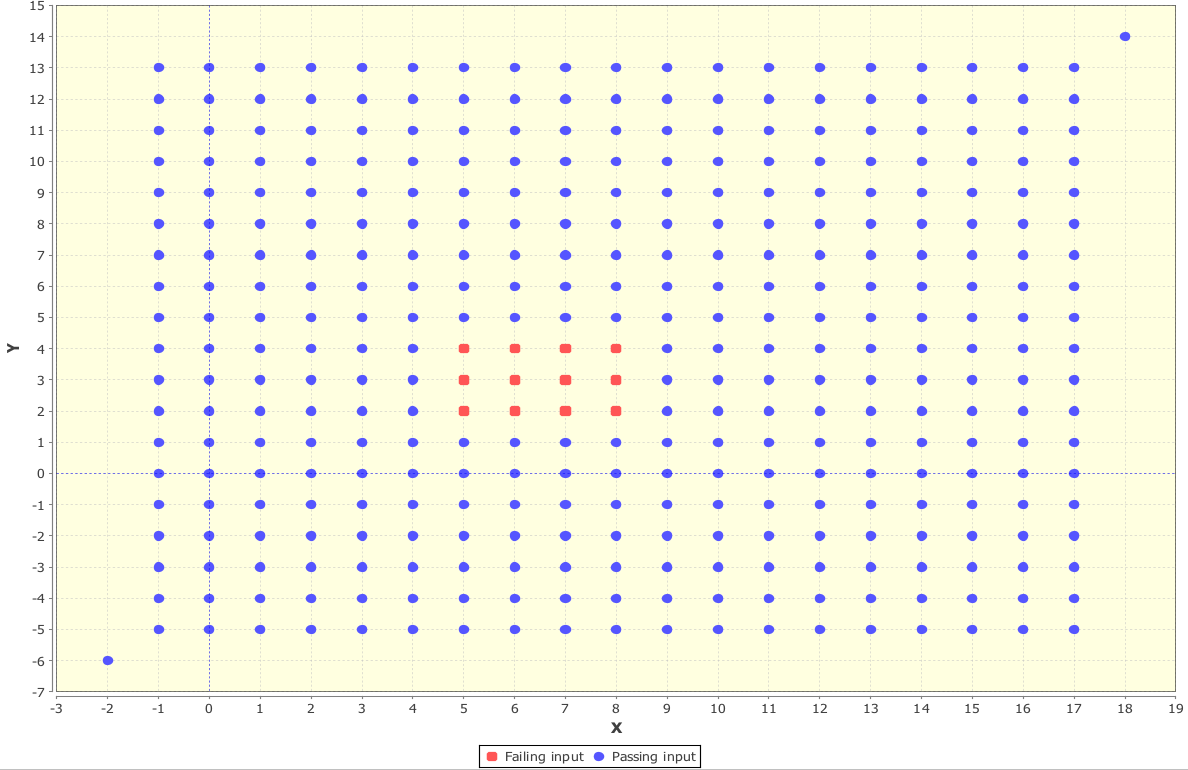
\includegraphics[width=14cm,height=6.2cm]{chapter6/BFDTwo.png}
\label{fig:BFDOne}
}
\subfigure[Strip failure domain in two-dimension]{
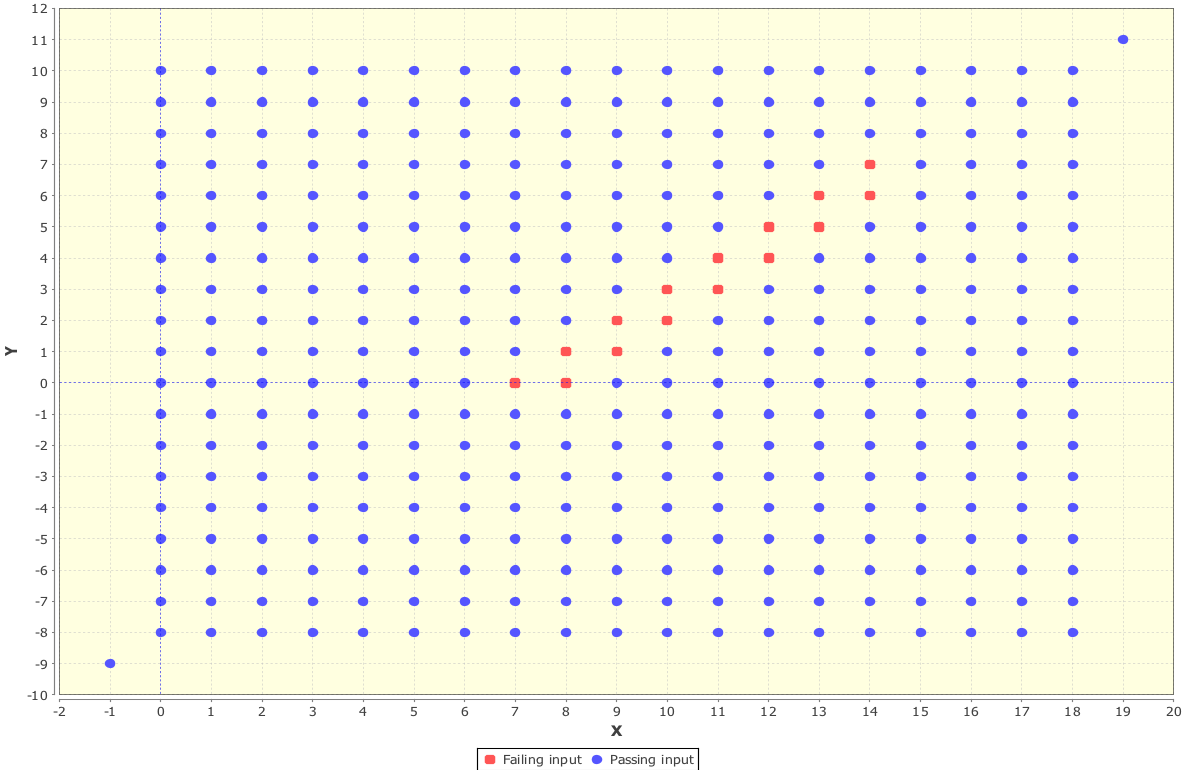
\includegraphics[width=14cm,height=6.2cm]{chapter6/SFDTwo.png}
\label{fig:SFDOne}
}
\caption{Pass and fail values plotted by ADFD+ for two-dimension programs}

\label{fig:failureDomainsTwoDimension_6}
\end{figure}


\begin{table}[h]
\caption{Table depicting values of x and y arguments responsible for forming point, block and strip failure domain in Figure \ref{fig:failureDomainsTwoDimension_6}}
\bigskip
\centering
{\renewcommand{\arraystretch}{1.3}
\begin{tabular}{|l|l|l|}
\hline
Point failure		& 	Block failure		& 	Strip failure		\\
\hline
x = 2, y = 10	&	x = 5, y = 2		&	x = 7,~~y = 0	\\	
x = 4, y = 10	&	x = 6, y = 2		&	x = 8,~~y = 0	\\	
x = 7, y = 10	&	x = 7, y = 2		&	x = 8,~~y = 1	\\
x = 9, y = 10	& 	x = 8, y = 2 		& 	x = 9,~~y = 1	\\
				& 	x = 5, y = 3 		& 	x = 9,~~y = 2	\\
				& 	x = 6, y = 3 		& 	x = 10, y = 2	\\
				& 	x = 7, y = 3 		& 	x = 10, y = 3	\\
				& 	x = 8, y = 3 		& 	x = 11, y = 3	\\
				& 	x = 5, y = 4 		& 	x = 11, y = 4	\\
				& 	x = 6, y = 4 		& 	x = 12, y = 4	\\
				& 	x = 7, y = 4 		& 	x = 12, y = 5	\\
				& 	x = 8, y = 4 		& 	x = 13, y = 6	\\
				&			      		& 	x = 14, y = 6	\\				
				&			      		& 	x = 14, y = 7	\\
\hline
\end{tabular}
}
\bigskip
\label{failureDomains_6}
\end{table}

\subsection{Test of Two-dimension Programs by Daikon}\label{sec:intro6_12}













\begin{table}[ht]
\caption{Table depicting values of failure points identified by ADFD+ Daikon}
\bigskip
\centering
{\renewcommand{\arraystretch}{1.3}
\begin{tabular}{|l|l|r|r|r|r|}
\hline
Technique 	& Dimension	& Test cases		& 	Point failure		& 	Block failure	& 	Strip failure	\\
\hline
ADFD+		& 	One				& N/A			& 					& 				&				\\
Daikon		& 	One				& 10			&					&				&				\\
Daikon		& 	One				& 20			&					&				&				\\
ADFD+		& 	Two				& N/A			&					&				&				\\
Daikon		& 	Two				& 10			&					&				&				\\
Daikon		& 	Two				& 20			&					&				&				\\
\hline
\end{tabular}
}
\bigskip
\label{table:ADFD+Results_6}
\end{table}




%for point, block and strip of one dimensional program. Use the same programs of ADFD, same figures but analyse it again on Daikon. because ADFD and ADFD+ behave in the same way for one dimension. For point block and strip of two dimensional programs. Use adfd+ system.






\section{Discussion}\label{sec:intro6_13}
We have shown that ADFD+ is a promising technique to find a failure and using it as a focal point find the whole failure domain. We have also shown that ADFD+ can graphically draw the failure domain on a chart. The failure values are drawn in red and the pass values are drawn in green. The pictorial representation of failure domain helps in easily identifying the underlying pattern and its boundaries.

As a pilot study, we also ran an empirical study to evaluate several error-seeded programs. While it would be surprising if production programs produced much different results, it would be worthwhile to check.

More importantly, the implementation of ADFD+ for this pilot study has significant limitations in practice, as it requires only one and two dimensional numerical programs. Though it is not difficult to extend the approach to test more than two-dimensional programs containing other primitive types, it would however be difficult to plot them on the chart as the number of coordinates increases. The approach can also be extended to test object-oriented programs by implementing objects distance proposed by Ciupa et al. \cite{ciupa2006object}. The details of such an implementation will take some effort.

The ADFD+ range value specifies how many values to test around the failure. The range can be set to any number before the test starts. The value of range is directly proportional to the time taken because the higher the range value the higher number of values to test. Higher range value also leads to a very large graph and the tester has to use the zoom feature of graph to magnify the failure region.




\section{Threats to Validity}\label{sec:intro6_14}
The research study faces threats to external and internal validity. The threats to external validity are the same, which are common to most of the empirical evaluations i.e. to what degree the classes under test and test generation tool (Randoop) are representatives of true practice. The classes under test contains failure patterns in only one and two-dimensional input domain. The threats may be reduced to a greater extent in future experiments by taking several types of classes and different test generation tools. 

The threat to internal validity includes annotation of invariants that can bias the results, which may have been caused by error-seeded classes used in our experiments. Internal threats may be avoided by taking real classes and failures in the experiments. Moreover, testing a higher number of classes will also increase the validity of the results.

\section{Conclusions}
Automated Discovery of Failure Domain+ (ADFD+) is distinctive from other random test strategies in the sense that it is not only limited to identifying a failure in the program. Instead, the failure is exploited to identify and graphically plot its failure domain.

In the first section, we describe ADFD+ in detail which is based on our previous approach ADFD~\cite{ahmad2013adfd}. We then describe the main improvements of ADFD+ over ADFD. 

In the second section, we analysed and compared the results of the experiments performed by both ADFD+ and Daikon in the case of programs with point, block and strip failure domain. 

We showed that Daikon lakes to accurately identify the failure boundary and therefore cannot generate invariants for such failures.  We further explain why Daikon does not work well for boundary failures. The main reason we identified for this behaviour is Daikons dependence on initial set of test cases, which are required by Daikon for generating invariants. With increase in number of test suite or high quality test suite improves the performance of invariants. 

\section{Future Work}\label{sec:intro6_15}
The current approach can be extended to a larger set of real world multi-dimensional programs, using real failure instead of error-seeded programs. However, to plot failure domains of complex multi-dimensional nature, more sophisticated graphical tools like Matlab will be required rathar than JFreeChart used in the current study. This may not restrict the formation of new failure domains to point, block and strip failure domain in one and two-dimensional numerical programs. 

